\begingroup
\let\figure\RSIappendixfigure
\let\endfigure\RSIendappendixfigure
\subsubsection{Block-level one-step errors and update projections}
\label{app:one-step-raw-figures}

Figures~\ref{fig:one-step-raw-qwen17}--\ref{fig:one-step-raw-llama}
show the original primary ID error-change and reference-projection plots
for the three completed one-step graph studies. These block-level views
complement the aggregate accuracy contrasts in
Figure~\ref{fig:one-step-contrasts} and Tables~\ref{tab:one-step-heldout}
and~\ref{tab:one-step-diagnostics}. Within each source plot, the left
panel connects $R/S$ observations from the same block; the right panel
shows the five paired $S-R$ differences and their mean with a descriptive
95\% block-$t$ interval. Null denotes the run's own unupdated adapter.
Error is $1-\mathrm{Pass@1}$, so its contrasts have the opposite sign
to accuracy contrasts. Projection is a first-order reference-loss
diagnostic, not a certified finite-step loss change or held-out task risk.
Original plots use separate vertical scales; no cross-model magnitude
comparison is inferred from their appearance.

\begin{figure}[H]
\centering
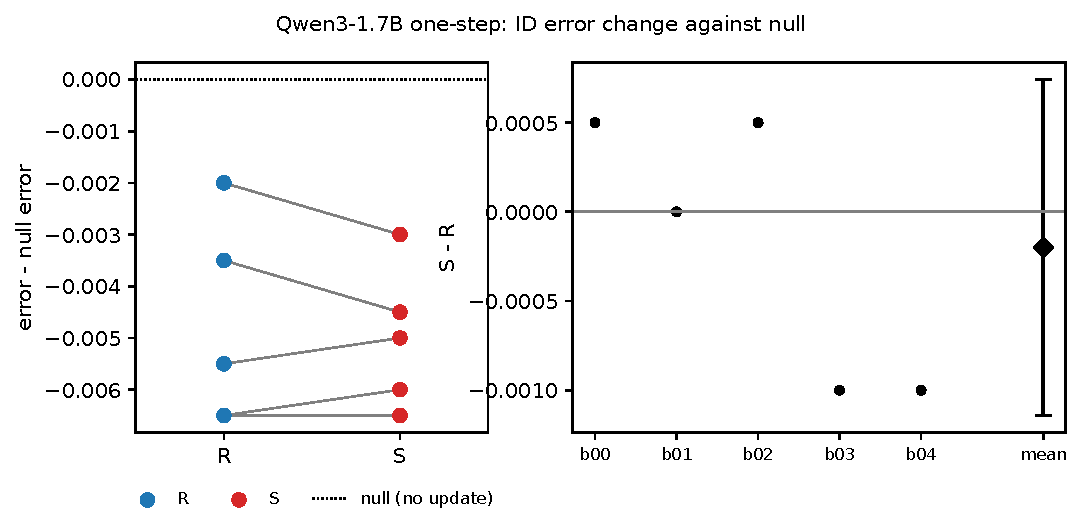
\includegraphics[width=0.82\linewidth]{figures/one_step_selected_raw/qwen3-1.7b_error_eval_id.pdf}
\par\smallskip
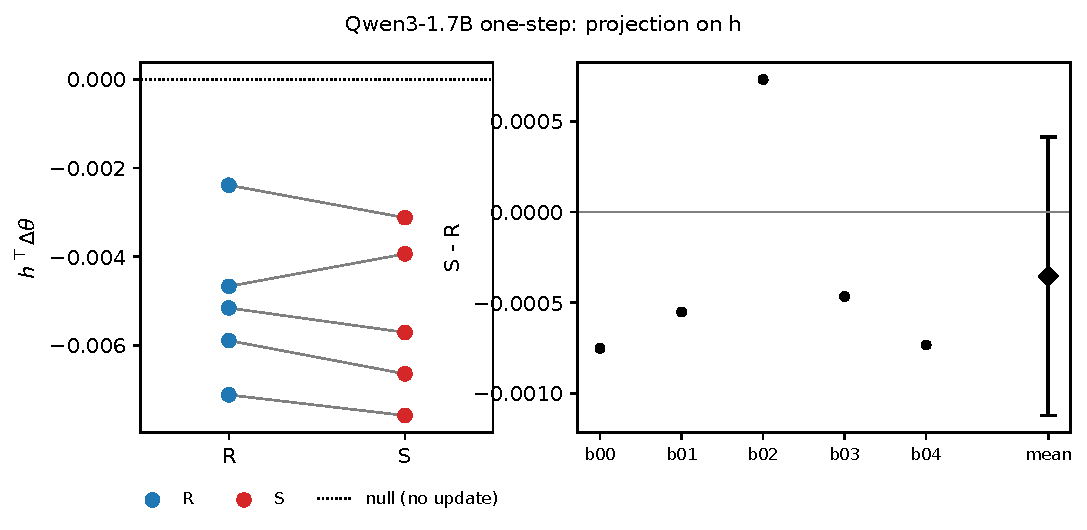
\includegraphics[width=0.82\linewidth]{figures/one_step_selected_raw/qwen3-1.7b_projection.pdf}
\caption{Original Qwen3-1.7B one-step ID error change against null
(top) and reference projection $h^T\Delta\theta$ (bottom), with five
paired blocks. The panels retain the run's own null as their reference.}
\label{fig:one-step-raw-qwen17}
\end{figure}

Both Qwen3-1.7B arms lower mean ID error relative to null, by
$0.0048/0.0050$ for $R/S$. The paired $S-R$ error contrast is
$-0.0002\pm0.0009$ and the projection contrast is
$-0.00035\pm0.00077$. Every block has
negative projection in both arms; none exhibits the theoretical
construction's opposite within-pair projection signs.

\begin{figure}[H]
\centering
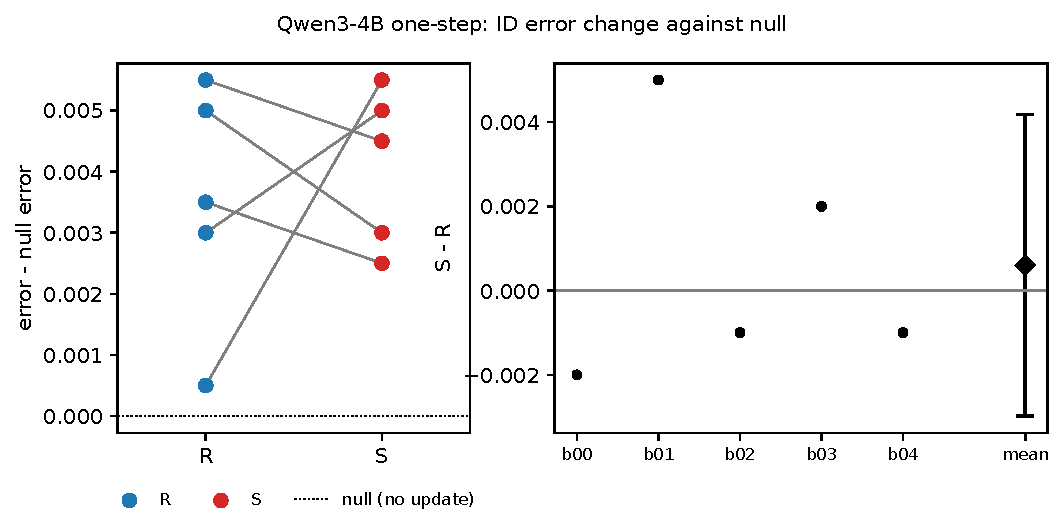
\includegraphics[width=0.82\linewidth]{figures/one_step_selected_raw/qwen3-4b_error_eval_id.pdf}
\par\smallskip
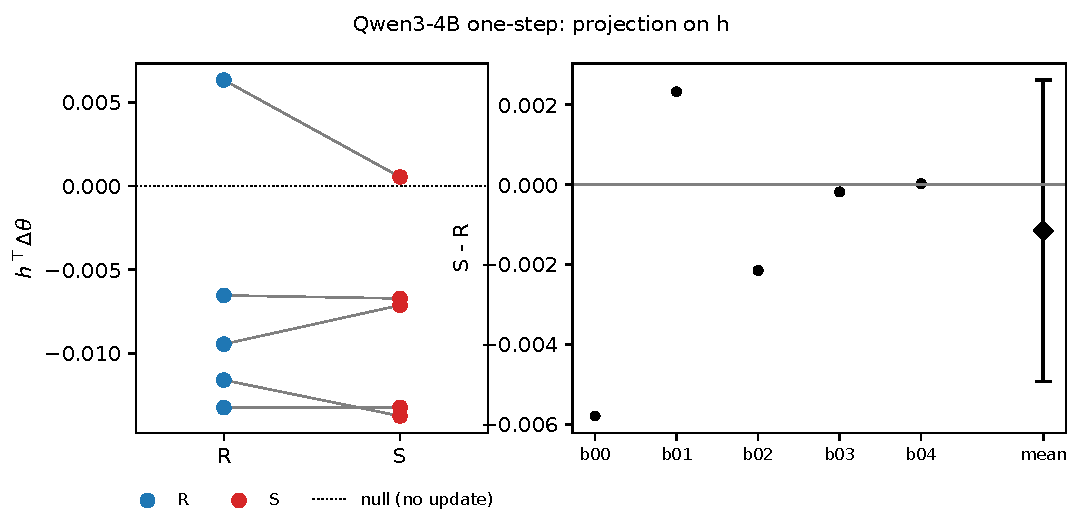
\includegraphics[width=0.82\linewidth]{figures/one_step_selected_raw/qwen3-4b_projection.pdf}
\caption{Original Qwen3-4B one-step ID error change against null
(top) and reference projection (bottom), with five paired blocks.
Error and projection are distinct outcomes and use separate scales.}
\label{fig:one-step-raw-qwen4}
\end{figure}

For Qwen3-4B, mean ID error increases by $0.0035/0.0041$ for $R/S$
despite negative mean projections. The paired contrasts are
$0.0006\pm0.0036$ for error and $-0.00115\pm0.00377$ for
projection. Block \texttt{b00} has positive
projection in both arms and the other four have negative projection
in both. A negative mean projection therefore does not certify
ID accuracy improvement.

\begin{figure}[H]
\centering
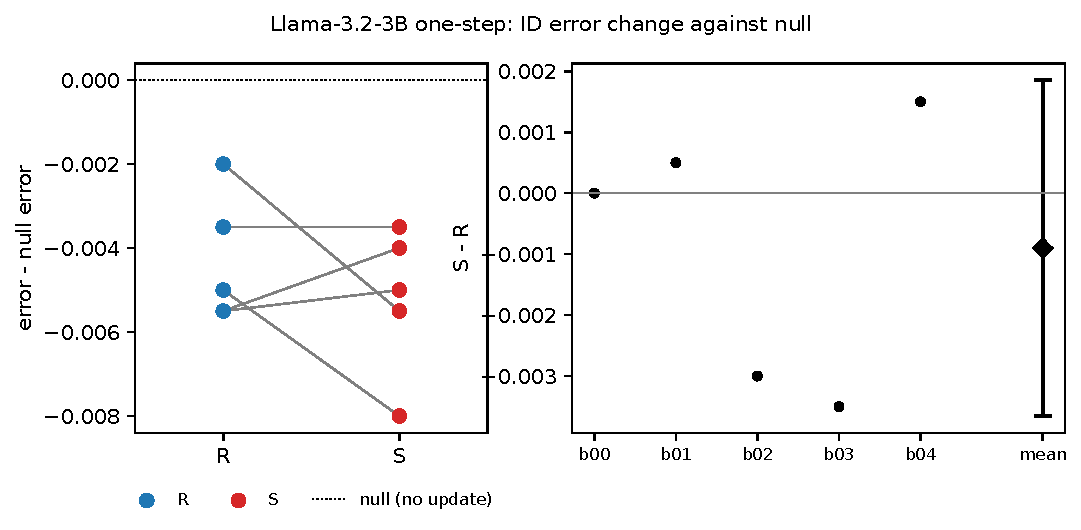
\includegraphics[width=0.82\linewidth]{figures/one_step_selected_raw/llama3.2-3b_error_eval_id.pdf}
\par\smallskip
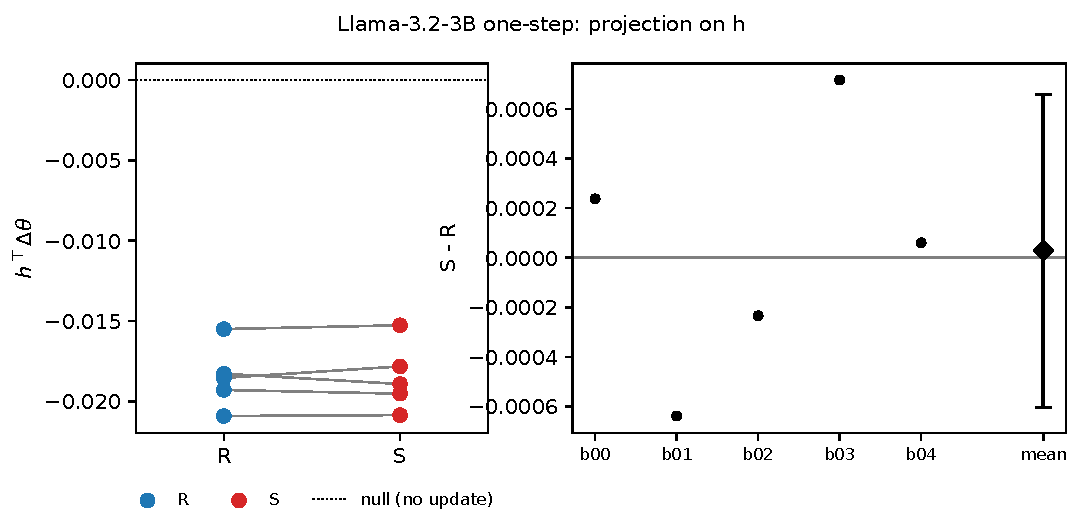
\includegraphics[width=0.82\linewidth]{figures/one_step_selected_raw/llama3.2-3b_projection.pdf}
\caption{Original Llama-3.2-3B-Instruct one-step ID error change
against null (top) and reference projection (bottom), with five
paired blocks.}
\label{fig:one-step-raw-llama}
\end{figure}

The Llama arms lower mean ID error by $0.0043/0.0052$ for $R/S$.
Paired contrasts are $-0.0009\pm0.0028$ for error and
$0.00003\pm0.00063$ for projection.
Every block has negative projection in both arms. These findings
do not establish equivalence of the arms or a within-pair directional
separation.
\endgroup
